\documentclass[10pt,fleqn]{article} % Default font size and left-justified equations
\usepackage[%
    pdftitle={Modélisation systèmes multiphysiques : Modélisation linéaire et non linéaire},
    pdfauthor={Xavier Pessoles}]{hyperref}
    
\input{style/new_style}
\input{style/macros_SII}
\usepackage{multicol}
\usepackage{siunitx}
\usepackage{picins}
\fichetrue
%\fichefalse

\proftrue
%\proffalse

\tdtrue
%\tdfalse

\courstrue
\coursfalse

\def\discipline{Sciences \\Industrielles de \\ l'Ingénieur}
\def\xxtete{Sciences Industrielles de l'Ingénieur}

\def\classe{PSI$\star$ -- MP}
\def\xxnumpartie{Cycle 01}
\def\xxpartie{Modéliser le comportement linéaire et non linéaire des systèmes multiphysiques}


\def\xxnumchapitre{Chapitre 1 \vspace{.2cm}}
\def\xxchapitre{\hspace{.12cm} Modélisation multiphysique}


\def\xxtitreexo{Actionneur électromécanique de la tuyère du lanceur européen VEGA}%Motorisation du moteur Haibike}
\def\xxsourceexo{\hspace{.2cm} \footnotesize{A. Caignot, V. Boyer, F. Golanski, D. Iceta, X. Pessoles, D. Violeau, Éd Vuibert.}}


\def\xxposongletx{2}
\def\xxposonglettext{1.45}
\def\xxposonglety{20}
%\def\xxonglet{Part. 1 -- Ch. 3}
\def\xxonglet{Cycle 01}

\def\xxactivite{TD 02}
\def\xxauteur{\textsl{A. Caignot, F. Golanski, F. Hospital, D. Iceta, X. Pessoles, D. Violeau, Éd Vuibert.}}

\def\xxcompetences{%
\textsl{%
\textbf{Savoirs et compétences :}\\
%Les sources sont associées par un \emph{hacheur série}. La détermination des grandeurs électriques associées à ce montage permet de conclure vis à vis du cahier des charges.
%\noindent \textbf{Résoudre :} à partir des modèles retenus :
%\begin{itemize}[label=\ding{112},font=\color{ocre}] 
%\item choisir une méthode de résolution analytique, graphique, numérique;
%\item mettre en \oe{}uvre une méthode de résolution.
%\end{itemize}
%\begin{itemize}[label=\ding{112},font=\color{ocre}] 
%\item \textit{Rés -- C1.1 :} Loi entrée sortie géométrique et cinématique -- Fermeture géométrique.
%\end{itemize}
%
%\noindent \textit{Mod2 -- C4.1 :} Représentation par schéma bloc.
}}

\def\xxfigures{
\includegraphics[width=.9\linewidth]{images/fig_01}
}%figues de la page de garde


\def\xxpied{%
Cycle 01 -- Modéliser le comportement des systèmes multiphysiques\\
Chapitre 1 -- \xxactivite%
}

\setcounter{secnumdepth}{5}
%---------------------------------------------------------------------------

\usepackage{pgfplots}
\begin{document}
\def\pathfig{images}
%\chapterimage{png/Fond_Cin}
\input{style/new_pagegarde}
\vspace{8cm}
\pagestyle{fancy}
\thispagestyle{plain}

\def\columnseprulecolor{\color{ocre}}
\setlength{\columnseprule}{0.4pt} 

\def\pathfig{images}

\begin{multicols}{2}



\section*{Analyser l'actionneur \\}





Le développement du lanceur européen VEGA a démarré en 1998 et s'est achevé en 2011. Ce projet répondait à une demande de mise en orbite basse et polaire, à coûts réduits, de satellites scientifiques dont la masse peut aller jusqu'à \SI{2 000}{kg}. La minimisation des coûts s'est appuyée sur l'intégration de technologies avancées déjà disponibles et l'utilisation des installations des lanceurs Ariane.

%\piccaption{Lanceur européen VEGA et son actionneur électromécanique d'orientation de la poussée vectorielle du premier étage de propulsion.}

\begin{center}
\includegraphics[width=.95\linewidth]{images/fig_01}
\end{center}

%\parpic[r]{\begin{tikzpicture}
%\node at (0,0) {\includegraphics[width=2.5cm]{\pathfig/Image1_}};
%\node[scale=.6,align=center,right] at (0.35,-.7) {Point de rotulage équivalent};
%\node[scale=.6,align=center,left] at (-1.2,-1.35) {1\ier ~étage de \\ propulsion};
%\node[scale=.6,align=center,left] at (-.85,-1.85) {Tuyère};
%\node[scale=.6,align=center,right] at (1.2,-1.2) {Accrochage};
%\node[scale=.6,align=center,right] at (.9,-1.7){Actionneur\\ électromécanique};
%\node[scale=.6,align=center,right] at (1.1,-2.2) {Accrochage};
%\node[scale=.6,align=center,right] at (0.3,-2.6) {$\pm\SI{5.5}{\degree}$};
%\label{vega_1}
%\end{tikzpicture}
%}
Une des innovations de ce projet concerne le système de contrôle vectoriel de poussée (en anglais : <<~Thrust Vector Control~>>) du premier étage de propulsion P80. D'une longueur de dix mètres, le P80 est chargé de 88 tonnes de propergol solide. Ceci lui permet de disposer d'une poussée maximale de \SI{3 000}{kN} et d'un temps de combustion de 107 secondes. Alors que sur Ariane 5 le pilotage vectoriel de la poussée est assuré par des dispositifs à source de puissance hydraulique, sur le P80 cette tâche est assurée par des dispositifs à source de puissance électrique (en anglais : <<~Power By Wire~>>).

La tuyère est reliée à l'étage de propulsion, par une liaison qui permet de l'orienter autour du point fixe nommé <<~point de rotulage~>>. 


\subsection*{Cahier des charges\\}

Afin de bien contrôler la trajectoire de la fusée, il est indispensable d'orienter très rapidement et très précisément la tuyère. Le diagramme des exigences partiel de la figure suivante %\ref{p01_ex01_req} 
présente les valeurs des performances temporelles que doit réaliser l'actionneur.

\begin{center}
\includegraphics[width=.95\linewidth]{images/fig_02}
\textit{Diagramme partiel des exigences.}
\end{center}

%\begin{figure}[!ht]
%\centering
%%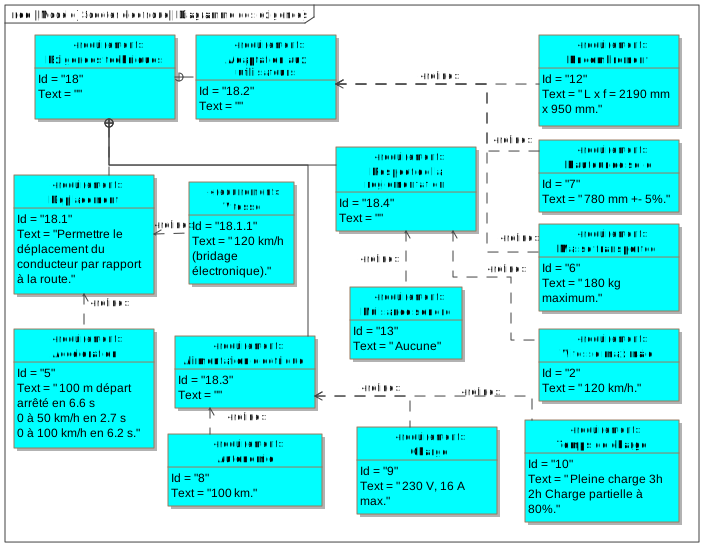
\includegraphics[width=.7\textwidth]{\pathfig/Exigences.png}
%
%\includestandalone[width=.7\textwidth]{\pathfig/Diagramme_exigences}
%\captionof{figure}{Diagramme partiel des exigences.}\label{p01_ex01_req}
%\end{figure}


%\subsection*{Problématique}

\begin{obj}
L'objectif est de vérifier les performances de rapidité et de précision décrites dans le diagramme des exigences. Un modèle multiphysique de l'actionneur va être mis en place afin de simuler le comportement de l'actionneur et de valider ou non son comportement vis-à-vis du cahier des charges. 
\end{obj}


\subsection*{Description structurelle\\} 
Les figures suivantes donnent la description des différents composants de l'actionneur.
%

\begin{center}
\includegraphics[width=.95\linewidth]{images/fig_03}
\textit{Diagramme de définition de blocs.}
\end{center}

\begin{center}
\includegraphics[width=.95\linewidth]{images/fig_04}
\textit{Diagramme de définition de blocs internes.}
\end{center}
%
%\begin{figure}[!ht]
%\centering
%%\includegraphics{\pathfig/Bdd.png}
%
%\includestandalone{\pathfig/Diagramme_bdd}
%\caption{Diagramme de définition de blocs.}
%\label{p01_ex01_bdd}
%\end{figure}
%
%
%
%\begin{figure}[!ht]
%\centering
%\includestandalone{\pathfig/Diagramme_IBD}
%
%%\includegraphics{\pathfig/Image22.pdf}
%\caption{Diagramme de blocs internes.}
%\label{p01_ex01_ibd}
%\end{figure}

\section*{Modéliser l'actionneur\\}



%\item En utilisant les informations données dans le diagramme IBD réaliser un diagramme de type "chaine d'information et chaine d'énergie". Identifier sur ce schéma les fonctions de chacun des composants de l'actionneur et les grandeurs physiques d'entrées/sorties correspondantes.
 



Afin de simuler le comportement dynamique de l'actionneur, il est nécessaire de représenter la charge qu'il devra mettre en mouvement. Pour un solide en rotation on parle d'inertie. Cette grandeur s'exprime en $\SI{}{kg. m^2}$ et quantifie la résistance d'un corps soumis à une accélération angulaire (le pendant de la masse qui caractérise la résistance d'un corps soumis à une accélération linéaire).
Un frottement visqueux de l'arbre moteur est ajouté %(Figure \ref{p01_ex_01_im3}) 
pour modéliser la manière dont est lubrifié le mécanisme.

%\textcolor{red}{ DV J'ai ajouté une petite explication de fv pour faciliter la suite. }




\begin{center}
\includegraphics[width=.95\linewidth]{images/fig_05}
\textit{Modèle à compléter.}
\end{center}
%

%
%\begin{figure}[!ht]
%\centering
%\includegraphics[width=12cm]{\pathfig/fig3_modif}
%\caption{Modèle à compléter.}
%\label{p01_ex_01_im3} 
%\end{figure}


\subparagraph{}\textit{En utilisant le diagramme IBD indiquer les noms des composants que représente chacun des blocs de la simulation. Identifier le bloc correspondant à la consigne et le bloc correspondant à la sortie. Quelles sont les unités de l'entrée et de la sortie?}
%
%\textcolor{red}{ DI remis la remarque de DV car pas prise en compte: DV Pas facile si on ne connait pas scilab mais très intéressant. Par contre je ne
%suis pas d’accord avec le corrigé. Je vois le bloc avt le moteur comme un variateur.
%Mais j’avoue que la consigne serait mieux en tension. Donc il faudrait mettre un
%seul bloc sous simm qui correspondrait à une tension créneau imposée quitte à
%changer à la main le symbole.}

\subparagraph{}\textit{ En utilisant les données du diagramme BDD indiquer les paramètres à renseigner dans chacun des blocs de la simulation.}
 
%\interenum{
Une simulation est réalisée pour une consigne de tension de \SI{200}{V}.
%Figure \ref{p01_ex_01_simu1}.


\begin{center}
\includegraphics[width=.95\linewidth]{images/fig_06}
\textit{Réponse à un échelon de 200 V du modèle.}
\end{center}
%
%
%\begin{figure}[!ht]
%\centering
%
%%\includegraphics[width=12cm]{\pathfig/fig4}
%\includestandalone{\pathfig/fig4_V2}
%\caption{Réponse à un échelon de 200 V du modèle.}
%\label{p01_ex_01_simu1} 
%\end{figure}}

\subparagraph{}\textit{ En analysant la réponse obtenue, que représente le $1$ dans le bloc << Time >> de la simulation ? Quelle est l'influence du frottement visqueux sur la rapidité de la réponse du système ?}

%\textcolor{red}{ DI remis la remarque de DV car pas prise en compte: DV Il faut refaire cette figure en mettant deux ou trois courbes correspondant à différentes valeurs de fv, ça permettra d'aider pour répondre à la dernière question. On fait une simul pour notamment voir l'influence du frottement visqueux sur la réponse. Si c'est ok, il faut ajouter une question : Quelle est l'influence du frottement visqueux sur la rapidité de la réponse du système ? }


\subparagraph{}\textit{ Peut-on, avec ce modèle, choisir une consigne angulaire en entrée et étudier les performances exigées dans le cahier des charges? Quels éléments du diagramme IBD n'ont pas été pris en compte dans ce modèle ?}

Afin de simplifier le modèle et les calculs, le moteur et le générateur sont remplacés par une source de couple. Le couple est l'action que produit le moteur sur son axe afin de le mettre en rotation.%M (Figure \ref{simpli}).

\begin{center}
\includegraphics[width=.95\linewidth]{images/fig_07}
\textit{Simplification de la partie électronique. }
\end{center}

%\begin{figure}[!ht]
%\includegraphics[width=6cm]{\pathfig/Image4}
%\caption{Simplification de la partie électronique. }
%\label{simpli}
%\end{figure}

De plus, le modèle simplifié de la figure est complété afin de modéliser la partie commande du système.% (Figure \ref{modSimpli}). 

\begin{center}
\includegraphics[width=.95\linewidth]{images/fig_08}
\textit{Modèle avec la partie commande.}
\end{center}
%
%\begin{figure}[!ht]
%\includegraphics[width=\textwidth]{\pathfig/repQ5_V2}
%\caption{Modèle avec la partie commande.}
%\label{modSimpli}
%\end{figure}



\section*{Analyser les performances prévues par le modèle\\} 

Pour une consigne de \num{5.5} degrés le résultat de la simulation est donné sur la figure suivante.%\ref{p01_ex_01_im6}.


\begin{center}
\includegraphics[width=.95\linewidth]{images/fig_09}
\textit{Réponse de l'actionneur sans saturation.}
\end{center}
%
%\begin{figure}[!ht]
%%\includegraphics[width=.8\textwidth]{\pathfig/Image5}
%\includestandalone[scale=.8]{\pathfig/Image5}
%\caption{Réponse de l'actionneur sans saturation.}
%\label{p01_ex_01_im6}
%\end{figure}
%%\textcolor{red}{ DV Faire un zoom un peu moins long mais plus haut pour obtenir précisément le t5\% }
%
%}
%




\subparagraph{}\textit{ Analyser le respect des exigences spécifiées dans le cahier des charges.}





\section*{Conclusion}
%\begin{conclusion}[ - Retour sur le cahier des charges]

Lors de la simulation précédente la tension maximale simulée dépasse la tension maximale admissible de $\SI{200}{V}$ du moteur réel. Afin de modéliser cette limite, un bloc (dit de <<~saturation~>> que l'on reverra dans le chapitre suivant) est placé en amont du moteur comme présenté figure suivante %\ref{p01_ex_01_im7}. 
Le comportement de ce bloc est simple:
\begin{itemize}
\item si la valeur absolue de la tension d'entrée $u$ du bloc est inférieure à $u_{\text{max}}$ alors la tension de sortie est égale à $u$;
\item si la valeur absolue de la tension d'entrée du bloc est supérieure à $u_{\text{max}}$ alors la tension de sortie est égale à $u_{\text{max}}$ si $u$ est positive (respectivement ($-u_{\text{max}}$ si $u$ est négative).
\end{itemize}
 
 \begin{center}
\includegraphics[width=.95\linewidth]{images/fig_10}
\textit{Modèle avec saturation.}
\end{center}

%\begin{center}
%\includegraphics[width=\linewidth]{\pathfig/Image7_01}
%%\includestandalone{\pathfig/Image7_02}
%%\includegraphics[width=.8\textwidth]{\pathfig/Image7}
%\captionof{figure}{Modèle avec saturation. \label{p01_ex_01_im7} }
%\end{center}


 \begin{center}
\includegraphics[width=.95\linewidth]{images/fig_11}
\textit{Simulation avec saturation.}
\end{center}

%\begin{center}
%%\includegraphics{\pathfig/Image7_01}
%\includestandalone{\pathfig/Image7_02}
%%\includegraphics[width=.8\textwidth]{\pathfig/Image7}
%\captionof{figure}{Simulation avec saturation. \label{p01_ex_01_im7bis}} \end{center}





\subparagraph{}\textit{Expliquer alors l'allure de la réponse figure ci-dessus.%Figure \ref{p01_ex_01_im7bis}. 
Le cahier des charges est-il toujours respecté ?}

\subparagraph{}\textit{Quel est l'écart relatif (en pourcentage) vis-à-vis du cahier des charges ?  En utilisant les analyses menées tout au long de l'exercice, indiquer quel paramètre permettrait de diminuer cet écart.}

%\textcolor{red}{ DI remis la remarque de DV car pas prise en compte: DV Je ne sais jamais trop comment faire un écart en pourcentage. J'ai ajouté par rapport aux valeurs du cahier des charges pour avoir unicité des réponses. }





\end{multicols}

\end{document}



%\begin{center}
%
%\includestandalone{\pathfig/Image7_02}
%\captionof{figure}{Simulation avec saturation \label{p01_ex_01_im7bis} }
%\end{center}





















\end{exoApp}




%%%%%%%%%%%%%%%%%%%%%%%%%%%%%%%%%%%%%%%
%%%%% CORRECTION
%%%%%%%%%%%%%%%%%%%%%%%%%%%%%%%%%%%%%%%

\begin{correction}

\def\pathfig{CHAP2/ex_vega/images}

\begin{questions}
%\item ~\\
%\begin{center}
%\includegraphics[width=\textwidth]{\pathfig/CECI}

%\captionof{figure}{Chaine d'énergie et d'information}
%\end{center}

\item Les éléments du modèle sont identifiés sur la figure \ref{Reponse2}. Il suffit d'observer le symbole utilisé dans chaque bloc pour en déduire le nom du constituant physique, même sans connaître précisément le logiciel utilisé pour réaliser ce modèle multiphysique.

\item Les paramètres à renseigner pour chaque bloc sont indiqués sur la figure \ref{Reponse2}. Il y a correspondance directe entre les paramètres nécessaires pour les modèles et ceux donnés dans le diagramme BDD.

\begin{figure}[!ht]
\centering
\includestandalone[width=.9\textwidth]{\pathfig/Reponse2_V2}
\caption{Diagramme de simulation complété.}
\label{Reponse2}
\end{figure}

%\begin{figure}[!ht]
%\centering
%\includegraphics[width=\textwidth]{\pathfig/repQ4_V2}
%\caption{Modèle Scilab SIMM}
%\label{Reponse3}
%\end{figure}

%\item  ~\\
%\begin{center}
%\includegraphics[width=\textwidth]{\pathfig/repQ5_V2}
%\captionof{figure}{Modèle asservi}
%\end{center}

\item Le bloc << Time >> permet de renseigner le temps durant lequel on cherche à déterminer l'évolution de la sortie.
Plus le frottement visqueux est grand, moins le système sera rapide (la pente de la courbe de position angulaire est plus petite donc la vitesse plus petite). 


\item  L'entrée est ici la consigne en volt fournie au moteur. Il n'est donc pas possible de choisir une consigne angulaire. Il manque dans le modèle la partie commande ainsi que le variateur de vitesse bien que l'on puisse interpréter le bloc d'entrée comme un variateur qui prend en entrée un signal et donne en sortie une tension.

%\textcolor{red}{ DV si on change les 2 blocs avant le moteur en 1 seul bloc, sinon il y a le variateur car entrée signal sortie tension.}

%\item La boucle de retour récupère l'information de position angulaire fournie par le capteur. Cette information est comparée (bloc comportant un sigma majuscule) avec la valeur de consigne angulaire fixée dans le bloc en haut à gauche du schéma. L'écart obtenu est alors amplifié par un gain constant de 400. La consigne est donc une position angulaire en degré (il faut qu'elle soit de même nature que la sortie pour que la comparaison puisse être effectuée).


\item  Le temps de réponse à $5 \%$ est inférieur à \SI{1}{ms} et l'écart statique est inférieur à 0,05\textdegree. Les critères du cahier des charges sont donc vérifiés. 

%\begin{center}
%
%\captionof{figure}{Réponse de l'actionneur sans saturation}
%\end{center}

\item  La saturation de tension limite la vitesse de rotation du moteur qui ne peut pas accélérer aussi vite que le souhaiterait l'asservissement. Ainsi, le système met plus de temps pour atteindre la consigne demandée.
Le cahier des charges n'est plus respecté au niveau de la rapidité car le temps de réponse est alors de $\SI{0,16}{s}$ (voir Figure \ref{vega_R6}). 

\begin{figure}[!ht]
\centering
%\includegraphics[width=.8\textwidth]{\pathfig/repQ7}
\includestandalone{\pathfig/Image7_02_Corr}
\caption{Réponse de l'actionneur avec saturation.}
\label{vega_R6}
\end{figure}

 \enlargethispage{1em}
 
\item L'écart est de 220 \%... notre modélisation n'est donc pas validée car beaucoup trop loin de la réalité et de la performance de rapidité espérée. Afin d'améliorer la rapidité de notre modèle il suffit de diminuer les frottements visqueux (comme observé précédemment à la question 3). Il faut cependant prendre un coefficient de frottements visqueux très faible, de l'ordre de $\SI{0,01}{N.m.s.rad^{-1}}$.




%\begin{center}
%
%\includestandalone{\pathfig/repQ8}
%\captionof{figure}{\'Evolution de l'angle de la tuyère avec un coefficient de $\SI{0,01}{Nm s rad^{-1}}$}
%\end{center}

\end{questions}
\end{correction}



\end{multicols}



\end{document}